\newsection{2} {Boundary Value Problems and Fourier Expansions}
{Fourier Expansions I}
\currentpdfbookmark{Section 11.2 Fourier Expansions I}{section:11.2}
\vskip14pt

\renewcommand{\thissection}{\sectiontitle
{\,FOURIER EXPANSIONS I\quad}}
\thissection

\noindent
In Example~\ref{example:11.1.4} and
Exercises~11.1.~\hspace*{-3pt}\ref{exer:11.1.4}--11.1.~\hspace*{-3pt}\ref{exer:11.1.22} we saw
that the
  eigenfunctions of Problem~5 are orthogonal on $[-L,L]$ and the
eigenfunctions of Problems~1--4 are orthogonal on $[0,L]$.
In this section and the next we introduce some series expansions
in terms of these eigenfunctions.
We'll use these expansions  to solve partial differential equations in
Chapter~12.

\begin{theorem}\color{blue} \label{thmtype:11.2.1}
Suppose the functions  $\phi_1,$ $\phi_2,$
$\phi_3,$ \dots$,$ are orthogonal on $[a,b]$ and
\begin{equation} \label{eq:11.2.1}
\int_a^b\phi_n^2(x)\,dx\ne0,\quad n=1,2,3,\dots.
\end{equation}
Let $c_1,$ $c_2,$ $c_3,$\dots  be constants such that the partial sums
$f_N(x)=\sum_{m=1}^N c_m\phi_m(x)$ satisfy the inequalities
$$
|f_N(x)|\le M,\quad a\le x\le b,\quad N=1,2,3,\dots
$$
for some constant $M<\infty.$ Suppose  also that
the series
\begin{equation} \label{eq:11.2.2}
f(x)=\sum_{m=1}^\infty c_m\phi_m(x)
\end{equation}
converges and is integrable on $[a,b]$.
Then
\begin{equation} \label{eq:11.2.3}
c_n={\dst\int_a^bf(x)\phi_n(x)\,dx\over\dst\int_a^b\phi_n^2(x)\,dx},\quad
n=1,2,3,\dots.
\end{equation}
\end{theorem}

\proof Multiplying \eqref{eq:11.2.2} by $\phi_n$ and
integrating yields
\begin{equation} \label{eq:11.2.4}
\int_a^b f(x)\phi_n(x)\,dx=\int_a^b
\phi_n(x)\left(\sum_{m=1}^\infty c_m\phi_m(x)\right)\,dx.
\end{equation}
It can be shown that the
 boundedness of the partial sums
$\{f_N\}_{N=1}^\infty$ and the integrability of $f$
allow us to interchange the operations of integration and summation
on the right of \eqref{eq:11.2.4}, and rewrite \eqref{eq:11.2.4} as
\begin{equation} \label{eq:11.2.5}
\int_a^b f(x)\phi_n(x)\,dx=\sum_{m=1}^\infty c_m
\int_a^b\phi_n(x) \phi_m(x)\,dx.
\end{equation}
(This isn't  easy to prove.) Since
$$
\int_a^b\phi_n(x)\phi_m(x)\,dx=0\mbox{\quad if \quad}m\ne n,
$$
\eqref{eq:11.2.5} reduces to
$$
\int_a^bf(x) \phi_n(x)\,dx=c_n\int_a^b\phi_n^2(x)\,dx.
$$
Now  \eqref{eq:11.2.1} implies \eqref{eq:11.2.3}.\bbox

Theorem~\ref{thmtype:11.2.1} motivates the next
definition.

\begin{definition}\color{blue}\label{thmtype:11.2.2} \rm
Suppose
$\phi_1,$ $\phi_2$, \dots, $\phi_n$,\dots are
orthogonal on $[a,b]$ and
$\int_a^b\phi_n^2(x)\,dx\ne0$, $n=1$, $2$, $3$, \dots. Let
$f$ be integrable on $[a,b],$ and define
\begin{equation} \label{eq:11.2.6}
c_n={\dst\int_a^bf(x)\phi_n(x)\,dx\over\dst\int_a^b\phi_n^2(x)\,dx},\quad
n=1,2,3,\dots.
\end{equation}
Then the infinite series
$\sum_{n=1}^\infty c_n\phi_n(x)$ is called the {\color{blue}\it
Fourier expansion of $f$ in terms
of the orthogonal set\/} $\{\phi_n\}_{n=1}^\infty$, and
$c_1$, $c_2$, \dots, $c_n$, \dots
are called the {\color{blue}\it Fourier coefficients of $f$\/ with respect to\/}
$\{\phi_n\}_{n=1}^\infty$. We indicate the relationship between $f$
and its Fourier
 expansion by
\begin{equation} \label{eq:11.2.7}
f(x)\sim\sum_{n=1}^\infty c_n\phi_n(x),\quad  a\le x\le b.
\end{equation}
\end{definition}

You may wonder why we don't write
$$
f(x)=\sum_{n=1}^\infty c_n\phi_n(x),\quad  a\le x\le b,
$$
rather than \eqref{eq:11.2.7}.
Unfortunately, this isn't always true. The series on the right
may diverge for some or all values
of $x$ in $[a,b]$, or it may converge to $f(x)$ for some values of
$x$ and not for others.  So, for now,  we'll just think of the series
as being associated with $f$ because of the definition
of the coefficients $\{c_n\}$, and we'll indicate
this association informally as in \eqref{eq:11.2.7}.

\newpage
\boxit{Fourier Series}

\noindent
We'll now study Fourier expansions in terms
 of the eigenfunctions
$$
1,\, \cos{\pi x\over L},\, \sin{\pi x\over L},
\, \cos{2\pi x\over L}, \, \sin{2\pi x\over L},\dots,
\cos{n\pi x\over L}, \, \sin{n\pi x\over L},\dots.
$$
of Problem~5.
 If $f$ is integrable on $[-L,L]$,  its
Fourier expansion in terms of these functions is called the {\color{blue}\it
Fourier series of $f$ on $[-L,L]$\/}.  Since
$$
\int_{-L}^L 1^2\,dx=2L,
$$
$$
\int_{-L}^L\cos^2{n\pi x\over L}\,dx =
{1\over2}\int_{-L}^L\left(1+\cos{2n\pi x\over L}\right)\,dx=
{1\over2}\left(x+{L\over2n\pi}\sin{2n\pi x\over L}\right)
\lims{-L}L=L,
$$
and
$$
\int_{-L}^L\sin^2{n\pi x\over L}\,dx =
{1\over2}\int_{-L}^L\left(1-\cos{2n\pi x\over L}\right)\,dx=
{1\over2}\left(x-{L\over2n\pi}\sin{2n\pi x\over L}\right),
\lims{-L}L=L,
$$
we see from \eqref{eq:11.2.6} that the Fourier series of $f$ on $[-L,L]$ is
$$
 a_0+\sum_{n=1}^\infty \left(a_n\cos{n\pi x\over
L}+b_n\sin{n\pi x\over L}\right),
$$
where
$$
a_0={1\over 2L}\int_{-L}^L f(x)\,dx,
$$
$$
a_n= {1\over L}\int_{-L}^L f(x)\cos{n\pi
x\over L}\,dx,\mbox{\quad and \quad}
b_n={1\over L}\int_{-L}^L f(x)\sin{n\pi x\over L}\,dx,\,n\ge1.
$$

Note that
$a_0$ is the average value of $f$ on $[-L,L]$, while $a_n$ and $b_n$
(for $n\ge1$) are twice the average values of
$$
f(x)\cos{n\pi x\over L}\quad\mbox{ and }\quad f(x)\sin{n\pi x\over L}
$$
on $[-L,L]$, respectively.

\boxit{Convergence of Fourier Series}

\noindent
The  question of convergence of Fourier series for arbitrary
integrable functions is beyond the scope of this book. However, we can
state a theorem that settles this question for most functions that
arise in applications.

\begin{definition}\color{blue} \label{thmtype:11.2.3}\rm
A function  $f$ is said to be
  {\color{blue}\it piecewise smooth\/} on $[a,b]$ if:
\begin{alist}
\item % (a)
$f$ has at most finitely many points of discontinuity in $(a,b)$;
\item % (b)
$f'$ exists and is continuous except possibly at finitely many points
in $(a,b)$;
\item % (c)
$f(x_0+)=\lim_{x\to x_0+}f(x)$ and
$f'(x_0+)=\lim_{x\to x_0+}f'(x)$ exist if $a\le x_0<b$;
\item % (d)
$f(x_0-)=\lim_{x\to x_0-}f(x)$ and
$f'(x_0-)=\lim_{x\to x_0-}f'(x)$ exist if  $a< x_0\le b$.
\end{alist}
\end{definition}

Since $f$ and $f'$ are required to be continuous at all but
finitely many points in $[a,b]$,
 $f(x_0+)=f(x_0-)$
and $f'(x_0+)=f'(x_0-)$ for all but finitely many
values of $x_0$ in $(a,b)$. Recall from Section~8.1 that
$f$ is said to have a {\color{blue}\it jump discontinuity\/} at $x_0$
if $f(x_0+)\ne f(x_0-)$.

The next theorem gives sufficient conditions for convergence of a
Fourier series. The  proof is beyond the scope of this book.

\begin{theorem}\color{blue} \label{thmtype:11.2.4}
If $f$ is piecewise smooth on $[-L,L]$, then the Fourier series
\begin{equation} \label{eq:11.2.8}
F(x)=a_0+\sum_{n=1}^\infty\left(a_n\cos{n\pi x\over L}+b_n\sin{n\pi
x\over L}\right)
\end{equation}
of $f$
on $[-L,L]$ converges for all $x$ in $[-L,L];$ moreover$,$
$$
F(x)=
\left\{\begin{array}{cl}
f(x)&\mbox{if $-L<x<L$ and $f$ is continuous at $x$  }\\[2\jot]
\dst{f(x-)+f(x+)\over2}&\mbox{if $-L<x<L$ and $f$ is discontinuous at
$x$  }\\[2\jot]
\dst{f(-L+)+f(L-)\over2}&\mbox{if $x=L$ or $x=-L$.}
\end{array}\right.
$$
\end{theorem}

Since $f(x+)=f(x-)$ if $f$ is continuous at $x$, we can also say that
$$
F(x)=
\left\{\begin{array}{cl}
\dst{f(x+)+f(x-)\over2}&\mbox{if }-L<x<L,\\
\dst{f(L-)+f(-L+)\over2}&\mbox{if }x=\pm L.
\end{array}\right.
$$

Note that $F$ is itself  piecewise smooth on $[-L,L]$, and
 $F(x)=f(x)$ at all points in  the open interval
$(-L,L)$ where $f$ is continuous.
 Since the series in \eqref{eq:11.2.8}
converges to $F(x)$ for all $x$ in $[-L,L]$, you may be tempted to
infer
 that the error
$$
E_N(x)=
\left|F(x)-a_0-\sum_{n=1}^N\left(a_n\cos{n\pi x\over L}+b_n\sin{n\pi
x\over L}\right)\right|
$$
can be made as small as we please  for all $x$ in $[-L,L]$
by choosing $N$ sufficiently large. However, this isn't  true if
$f$ has a  discontinuity  somewhere in $(-L,L)$, or if $f(-L+)\ne
f(L-)$.  Here's  the situation in this case.

{\color{blue}\it
If $f$ has a jump discontinuity at a point $\alpha$ in $(-L,L)$,  there
will be sequences
of points $\{u_N\}$ and $\{v_N\}$ in $(-L,\alpha)$ and $(\alpha,L)$,
respectively, such that
$$
\lim_{N\to\infty}u_N=
\lim_{N\to\infty}v_N=\alpha
$$
and
$$
E_N(u_N)\approx .09|f(\alpha-)-f(\alpha+)|\mbox{\quad and \quad}
E_N(v_N)\approx .09|f(\alpha-)-f(\alpha+)|.
$$
Thus, the maximum value of the error $E_N(x)$ near $\alpha$ does not
approach zero as $N\to\infty$, but just occurs closer and closer to
$($and on both sides of\,$)$ $\alpha$, and is essentially independent
of
$N$.

If $f(-L+)\ne f(L-)$, then there will be sequences of points
 $\{u_N\}$ and $\{v_N\}$ in $(-L,L)$
such that
$$
\lim_{N\to\infty}u_N=-L,\quad
\lim_{N\to\infty}v_N=L,
$$
$$
E_N(u_N)\approx .09|f(-L+)-f(L-)|\mbox{\quad and \quad}
E_N(v_N)\approx .09|f(-L+)-f(L-)|.
$$}

This  is the
\href{http://www-history.mcs.st-and.ac.uk/Mathematicians/Gibbs.html}
{\color{blue}\it Gibbs
 phenomenon\/}. Having been alerted to
it, you may see it in Figures~\ref{figure:11.2.2}--\ref{figure:11.2.4},
 below;
however, we'll give a  specific example at the end of this section.

\begin{example}\label{example:11.2.1} \rm
Find the Fourier series of the piecewise smooth function
$$
f(x)=
\left\{\begin{array}{rlr}
-x,&-2< x<0,
\\{1\over2},&\phantom{-}0<x<2
\end{array}\right.
$$
on $[-2,2]$ (Figure~\ref{figure:11.2.1}). Determine the sum of
the Fourier series  for $-2\le x\le 2$.
\end{example}

\begin{figure}[tbp]
  \centering\color{blue}
  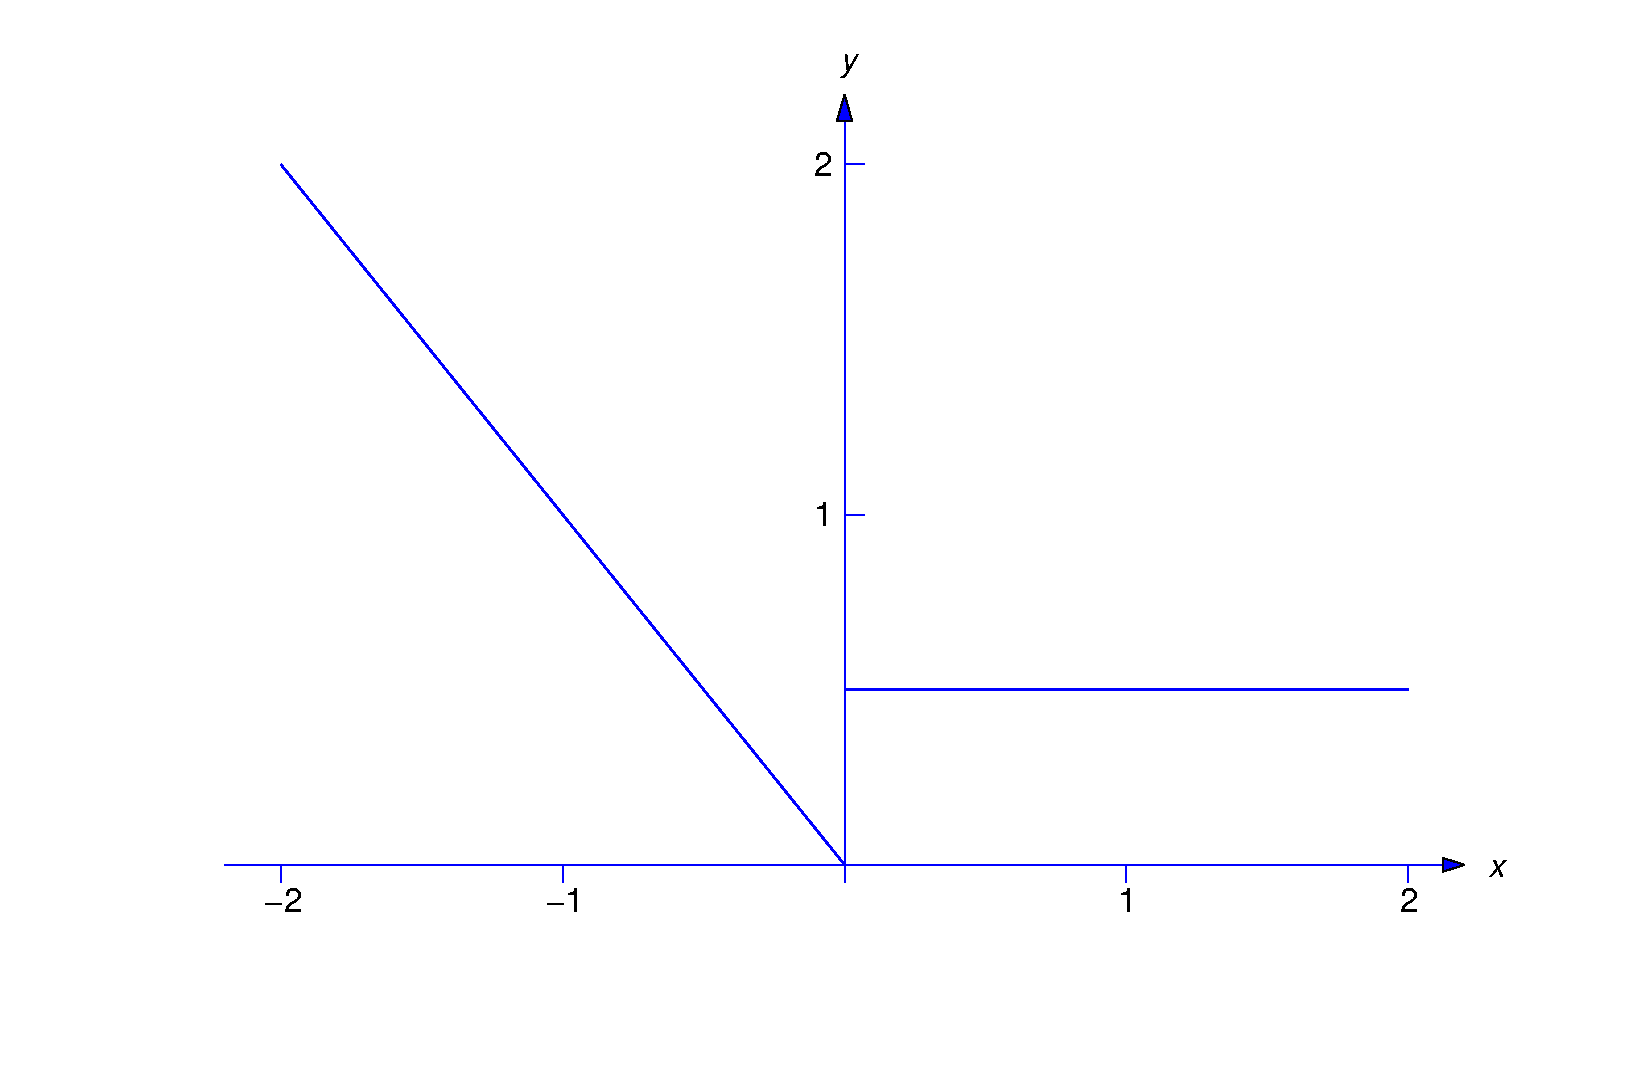
\includegraphics[bb=-78 148 689 643,width=5.67in,height=3.66in,keepaspectratio]{fig110201}
\caption{}
  \label{figure:11.2.1}
\end{figure}

\solution
Note that wen't bothered to define $f(-2)$, $f(0)$, and
$f(2)$.
 No matter
how they may be defined, $f$ is piecewise smooth on $[-2,2]$, and
the coefficients in the Fourier series
$$
F(x)=a_0+\sum_{n=1}^\infty\left(a_n\cos{n\pi
x\over2}+b_n\sin{n\pi x\over2}\right)
$$
are not affected by them. In any case,
Theorem~\ref{thmtype:11.2.4} implies that $F(x)=f(x)$ in $(-2,0)$
and $(0,2)$, where $f$ is continuous, while
$$
F(-2)=F(2)={f(-2+)+f(2-)\over2}=
{1\over2}\left(2+{1\over2}\right)={5\over4}
$$
and
$$
F(0)={f(0-)+f(0+)\over2}={1\over2}\left(0+{1\over2}\right)={1\over4}.
$$
To summarize,
$$
F(x)=
\left\{\begin{array}{rl}
{5\over4},&\phantom{-}x=-2\\[2\jot]
-x,&-2<x<0,\\[2\jot]
 {1\over4},&\phantom{-}x=0,\\[2\jot]
{1\over2},&\phantom{-}0<x<2,\\[2\jot]
{5\over4},&\phantom{-}x=2.
\end{array}\right.
$$

We compute the Fourier coefficients as follows:
$$
a_0={1\over4}\int_{-2}^2f(x)\,dx={1\over4}\left[\int_{-2}^0(-x)\,dx
+\int_0^2{1\over2}\,dx\right]
={3\over4}.
$$
If $n\ge1$, then
\begin{eqnarray*}
a_n&=&{1\over2}\int_{-2}^2f(x)\cos{n\pi
x\over2}\,dx={1\over2}\left[\int_{-2}^0(-x)\cos{n\pi x\over2}\,dx
+\int_0^2{1\over2}\cos{n\pi x\over2}\,dx\right]\\&=&{2\over
n^2\pi^2}(\cos n\pi-1),
\end{eqnarray*}
and
\begin{eqnarray*}
b_n&=&{1\over2}\int_{-2}^2f(x)\sin{n\pi
x\over2}\,dx={1\over2}\left[\int_{-2}^0(-x)\sin{n\pi x\over2}\,dx
+\int_0^2{1\over2}\sin{n\pi x\over2}\,dx\right]\\
&=&{1\over2n\pi}(1+3\cos n\pi).
\end{eqnarray*}
Therefore
$$
F(x)={3\over4}+{2\over\pi^2}\sum_{n=1}^\infty{\cos n\pi-1\over
n^2}\cos{n\pi x\over2}+{1\over2\pi}\sum_{n=1}^\infty{1+3\cos
n\pi\over n}\sin{n\pi x\over2}.
$$
Figure~\ref{figure:11.2.2} shows how the partial sum
$$
F_m(x)={3\over4}+{2\over\pi^2}\sum_{n=1}^m{\cos n\pi-1\over
n^2}\cos{n\pi x\over2}+{1\over2\pi}\sum_{n=1}^m{1+3\cos
n\pi\over n}\sin{n\pi x\over2}
$$
approximates $f(x)$ for $m=5$ (dotted curve), $m=10$  (dashed curve),
and $m=15$ (solid curve).

\begin{figure}[H]
  \centering\color{blue}
  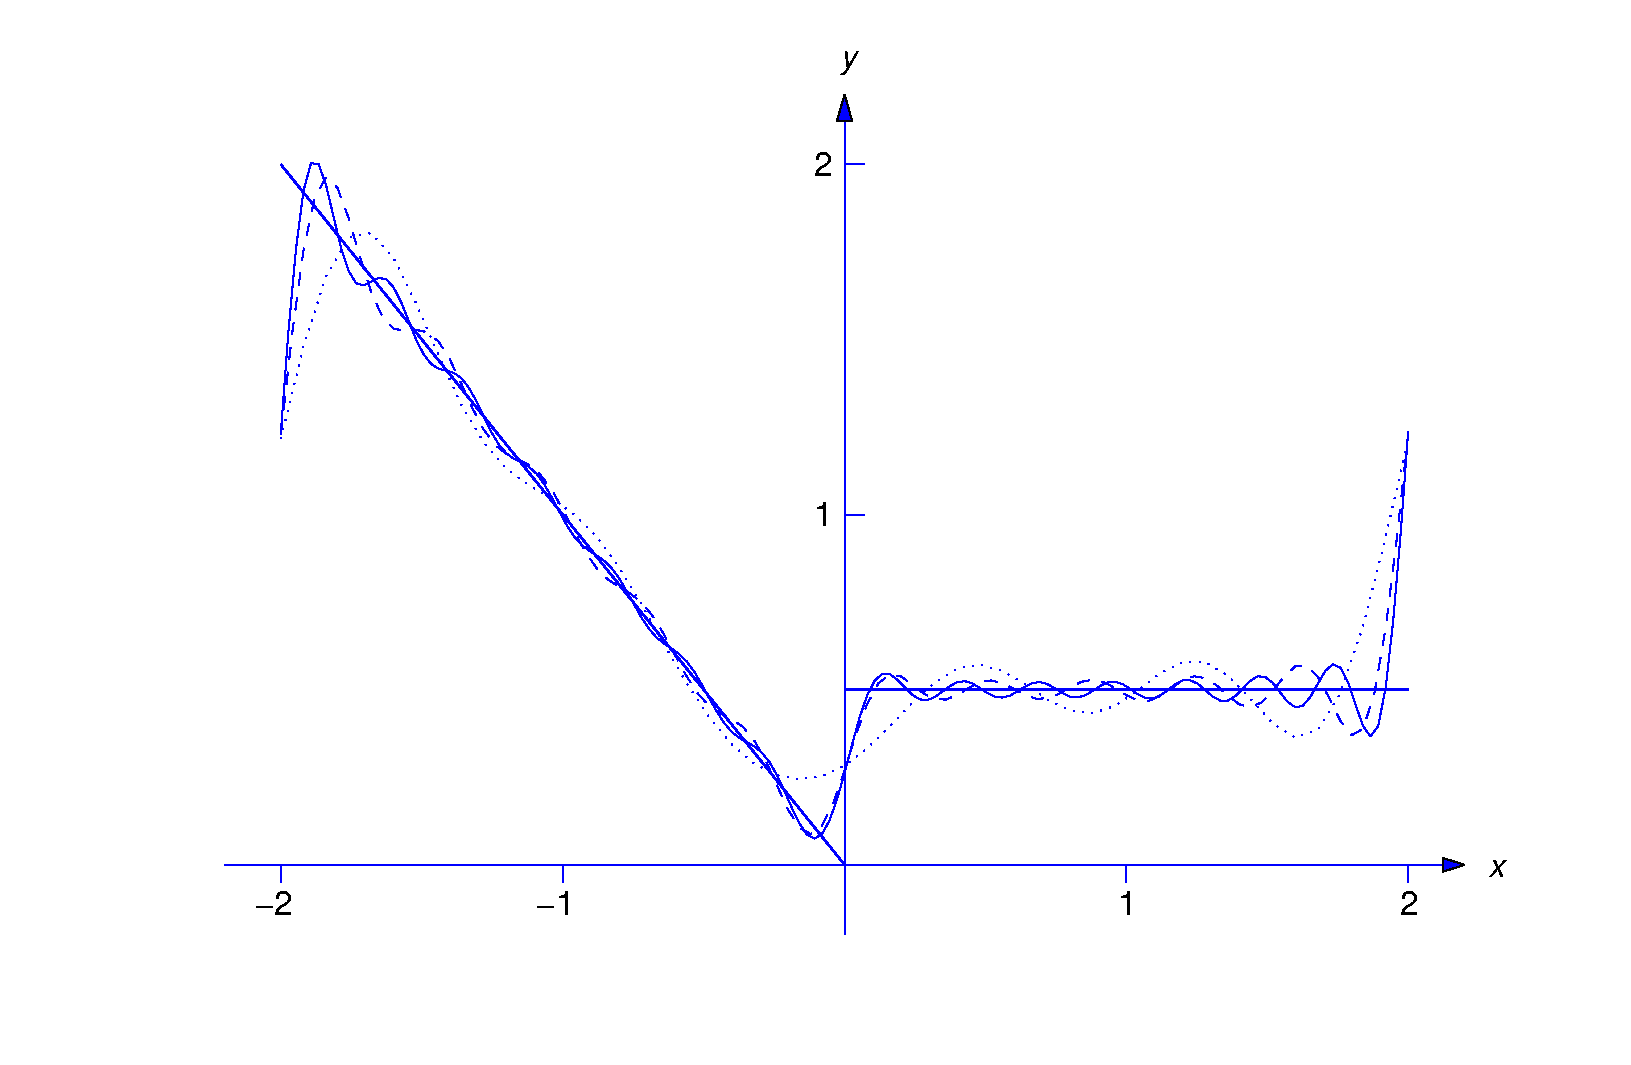
\includegraphics[bb=-78 148 689 643,width=5.67in,height=3.66in,keepaspectratio]{fig110202}
\caption{}
  \label{figure:11.2.2}
\end{figure}

\newpage
\boxit{Even and Odd Functions}

\noindent
Computing the Fourier coefficients of a  function  $f$
 can be tedious;     however,  the computation
can often be simplified by exploiting symmetries
in
$f$ or  some of its terms. To focus on this,
we recall some concepts that you studied in calculus.
Let $u$ and $v$ be defined on $[-L,L]$ and suppose
that
$$
u(-x)=u(x)\quad\mbox{ and }\quad v(-x)=-v(x),\quad -L\le x\le L.
$$
Then we say that $u$ is an {\color{blue}\it even\/} function and $v$  is an
{\color{blue}\it odd function\/}. Note that:
\begin{itemize}
\item
The product of two even functions is even.
\item
The product of two odd functions is even.
\item
The product of an even  function and an odd function  is odd.
\end{itemize}

\begin{example}\label{example:11.2.2} \rm
The functions $u(x)=\cos \omega x$ and $u(x)=x^2$  are even, while
$v(x)=\sin \omega x$ and $v(x)=x^3$ are odd. The function $w(x)=e^x$
is neither even nor odd.
\end{example}

You learned parts \part{a} and \part{b} of the  next theorem in
calculus, and the other parts follow from them
(Exercise~\ref{exer:11.2.1}).

\begin{theorem}\color{blue}\label{thmtype:11.2.5}
Suppose $u$ is even and $v$ is odd on $[-L,L].$ Then$:$
$$
\mbox{\part{a}\quad} \int_{-L}^L u(x)\,dx=2\int_0^Lu(x) \,dx,
\mbox{\quad  \part{b}\quad}
\int_{-L}^L v(x)\,dx=0,
$$
$$
\mbox{\part{c}\quad} \int_{-L}^L
u(x)\cos{n\pi x\over L}\,dx=2\int_0^Lu(x)\cos{n\pi x\over L} \,dx,
$$
$$
\mbox{\part{d}\quad}
\int_{-L}^L v(x)\sin{n\pi x\over L}\,dx=
2\int_0^L v(x)\sin{n\pi x\over L}\,dx,
$$
$$
\mbox{\part{e}\quad} \int_{-L}^L
u(x)\sin{n\pi x\over L}\,dx=0
\mbox{\quad and \quad\part{f}\quad}
\int_{-L}^L v(x)\cos{n\pi x\over L}\,dx=0.
$$
\end{theorem}

\begin{example}\label{example:11.2.3} \rm
Find the Fourier series of $f(x)=x^2-x$ on $[-2,2]$, and determine
its sum for $-2\le x\le 2$.
\end{example}

\solution Since $L=2$,
$$
F(x)=a_0+\sum_{n=1}^\infty\left(a_n\cos{n\pi
x\over2}+b_n\sin{n\pi x\over2}\right)
$$
where
\begin{equation} \label{eq:11.2.9}
a_0={1\over4}\int_{-2}^2(x^2-x)\,dx,
\end{equation}
\begin{equation} \label{eq:11.2.10}
a_n={1\over2}\int_{-2}^2(x^2-x)\cos{n\pi x\over2}\,dx,\quad
n=1,2,3,\dots,
\end{equation}
and
\begin{equation} \label{eq:11.2.11}
b_n={1\over2}\int_{-2}^2(x^2-x)\sin{n\pi x\over2}\,dx,\quad
n=1,2,3,\dots.
\end{equation}
We simplify the evaluation of these integrals by using
Theorem~\ref{thmtype:11.2.5}   with $u(x)=x^2$ and $v(x)=x$;
thus, from \eqref{eq:11.2.9},
$$
a_0={1\over2}\int_0^2x^2\,dx={x^3\over6}\lims02={4\over3}.
$$
From \eqref{eq:11.2.10},
\begin{eqnarray*}
a_n&=&\int_0^2x^2\cos{n\pi x\over2}\,dx=
{2\over n\pi}\left[x^2\sin{n\pi x\over2}\lims02-
2\int_0^2x\sin{n\pi x\over2}\,dx\right]\\
&=&{8\over n^2\pi^2}\left[x\cos{n\pi x\over2}\lims02-
\int_0^2\cos{n\pi x\over2}\,dx\right]\\
&=&{8\over n^2\pi^2}\left[2\cos n\pi-{2\over n\pi}\sin{n\pi
x\over2}\lims02\right]
=(-1)^n{16\over n^2\pi^2}.
\end{eqnarray*}
From \eqref{eq:11.2.11},
\begin{eqnarray*}
b_n&=&-\int_0^2x\sin{n\pi x\over2}\,dx
={2\over n\pi}\left[x\cos{n\pi x\over2}\lims02-
\int_0^2\cos{n\pi x\over2}\,dx\right]\\
&=&{2\over n\pi}\left[2\cos n\pi-{2\over
n\pi}\sin{n\pi x\over2}\lims02\right]=(-1)^n{4\over n\pi}.
\end{eqnarray*}
Therefore
$$
F(x)={4\over3}+{16\over\pi^2}\sum_{n=1}^\infty{(-1)^n\over n^2}
\cos{n\pi x\over2}+{4\over\pi}\sum_{n=1}^\infty
{(-1)^n\over n}\sin{n\pi x\over2}.
$$
Theorem~\ref{thmtype:11.2.4} implies that
$$
F(x)=
\left\{\begin{array}{cl}
4,&\phantom{-}x=-2,\\ x^2-x,&-2<x<2,\\4,&\phantom{-}x=2.
\end{array}\right.
$$
Figure~\ref{figure:11.2.3} shows how the partial sum
$$
F_m(x)={4\over3}+{16\over\pi^2}\sum_{n=1}^m{(-1)^n\over n^2}
\cos{n\pi x\over2}+{4\over\pi}\sum_{n=1}^m
{(-1)^n\over n}\sin{n\pi x\over2}
$$
approximates $f(x)$ for $m=5$ (dotted curve), $m=10$  (dashed curve),
and $m=15$ (solid curve).
\bbox

\begin{figure}[tbp]
  \centering\color{blue}
  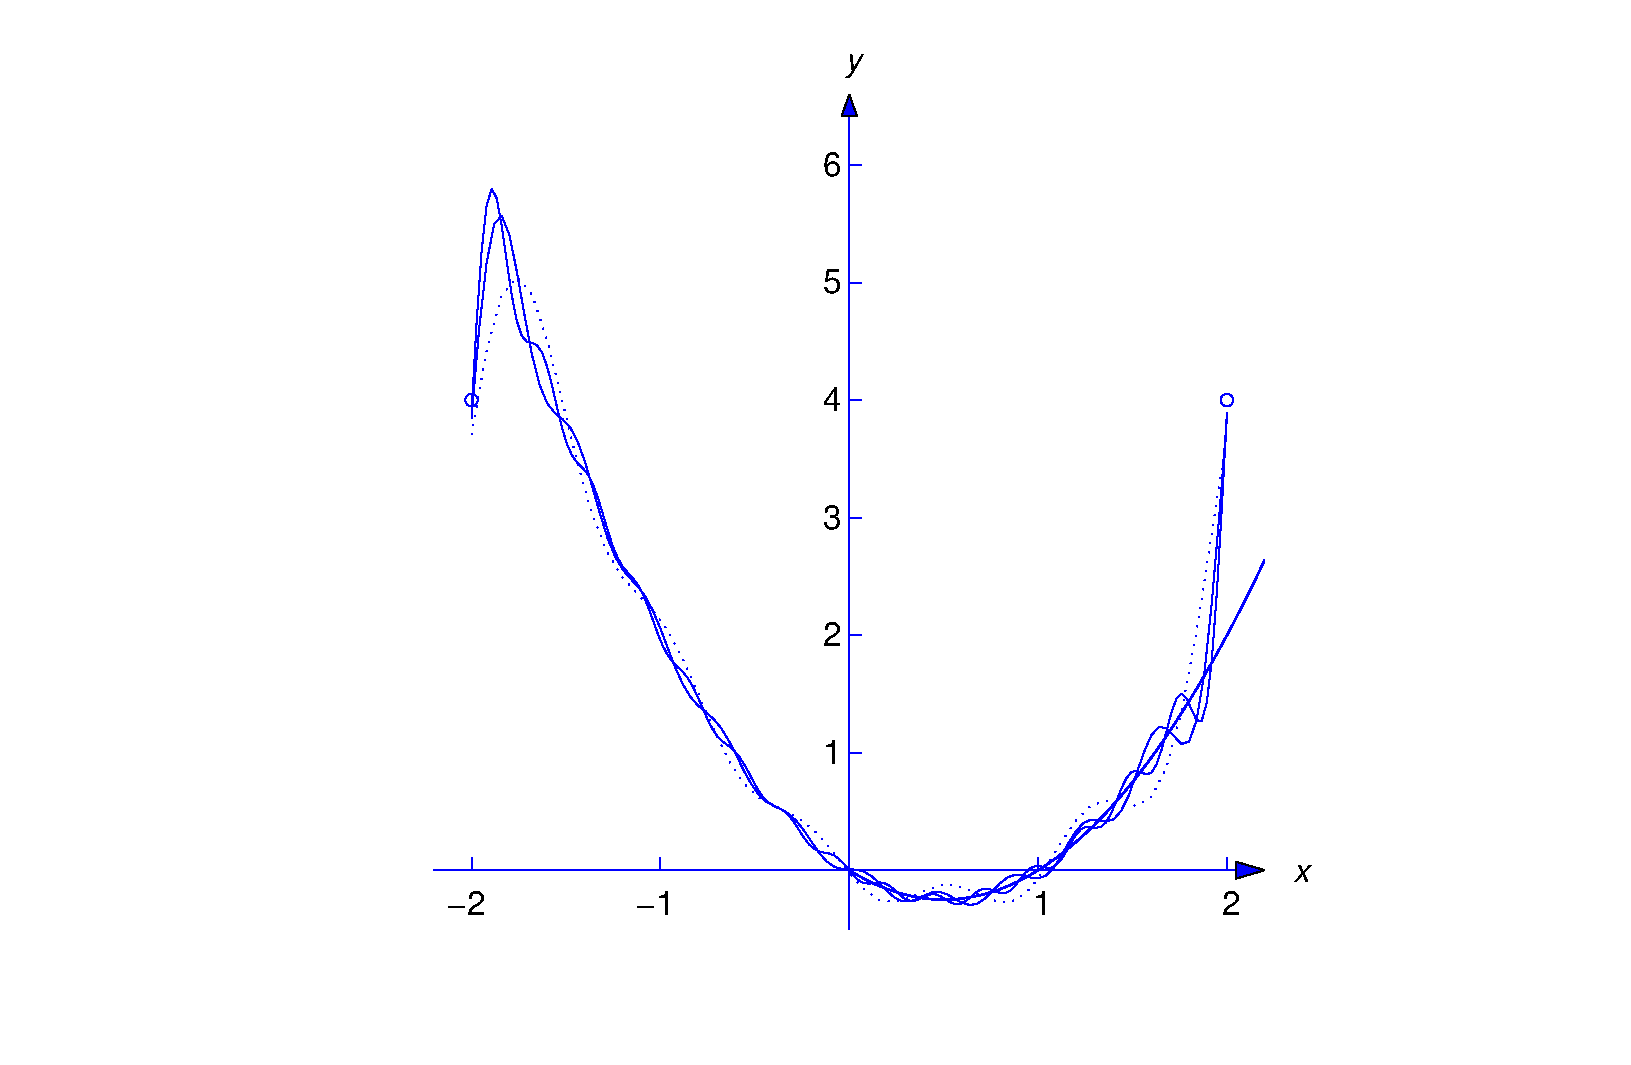
\includegraphics[bb=-78 148 689 643,width=5.67in,height=3.66in,keepaspectratio]{fig110203}
\caption{ Approximation of $f(x)=x^2-x$ by partial
sums of its Fourier series on $[-2,2]$}
  \label{figure:11.2.3}
\end{figure}

Theorem~\ref{thmtype:11.2.5} ilmplies
the next theorem follows.

\begin{theorem}\color{blue} \label{thmtype:11.2.6}
Suppose   $f$ is integrable on $[-L,L].$
\begin{alist}
\item % (a)
If $f$ is even$,$  the Fourier series of $f$ on $[-L,L]$ is
$$
F(x)=a_0+\sum_{n=1}^\infty a_n\cos{n\pi x\over L},
$$
where
$$
a_0={1\over L}\int_0^Lf(x) \,dx \mbox{\quad and \quad}
a_n={2\over L}\int_0^L f(x)\cos{n\pi x\over L}\,dx,\quad n\ge1.
$$
\item % (b)
If $f$ is odd$,$  the Fourier series of $f$ on $[-L,L]$ is
$$
F(x)= \sum_{n=1}^\infty b_n \sin{n\pi x\over L},
$$
where
$$
b_n={2\over L}\int_0^L f(x)\sin{n\pi x\over L}\,dx.
$$
\end{alist}
\end{theorem}

\begin{example}\label{example:11.2.4} \rm
Find the Fourier series of $f(x)=x$ on $[-\pi,\pi]$, and determine
its sum for $-\pi\le x\le \pi$.
\end{example}

\solution
Since $f$ is odd and $L=\pi$,
$$
F(x)=\sum_{n=1}^\infty b_n\sin nx
$$
where
\begin{eqnarray*}
b_n&=&{2\over\pi}\int_0^\pi x\sin nx\,dx=-{2\over
n\pi}\left[x\cos
nx\lims0\pi-\int_0^\pi\cos nx\,dx\right]\\
&=&-{2\over n}\cos n\pi+{2\over n^2\pi}\sin nx\lims0\pi=(-1)^{n+1}
{2\over n}.
\end{eqnarray*}
Therefore
$$
F(x)=-2\sum_{n=1}^\infty{(-1)^n\over n}\sin nx.
$$
Theorem~\ref{thmtype:11.2.4} implies that
$$
F(x)=
\left\{\begin{array}{cl}
0,&\phantom{-}x=-\pi,\\ x,&-\pi<x<\pi,\\0,&\phantom{-}x=\pi.
\end{array}\right.
$$
Figure~\ref{figure:11.2.4} shows how the partial sum
$$
F_m(x)=-2\sum_{n=1}^m{(-1)^n\over n}\sin nx
$$
approximates $f(x)$ for $m=5$ (dotted curve), $m=10$  (dashed curve),
and $m=15$ (solid curve).

\begin{figure}[tbp]
  \centering\color{blue}
  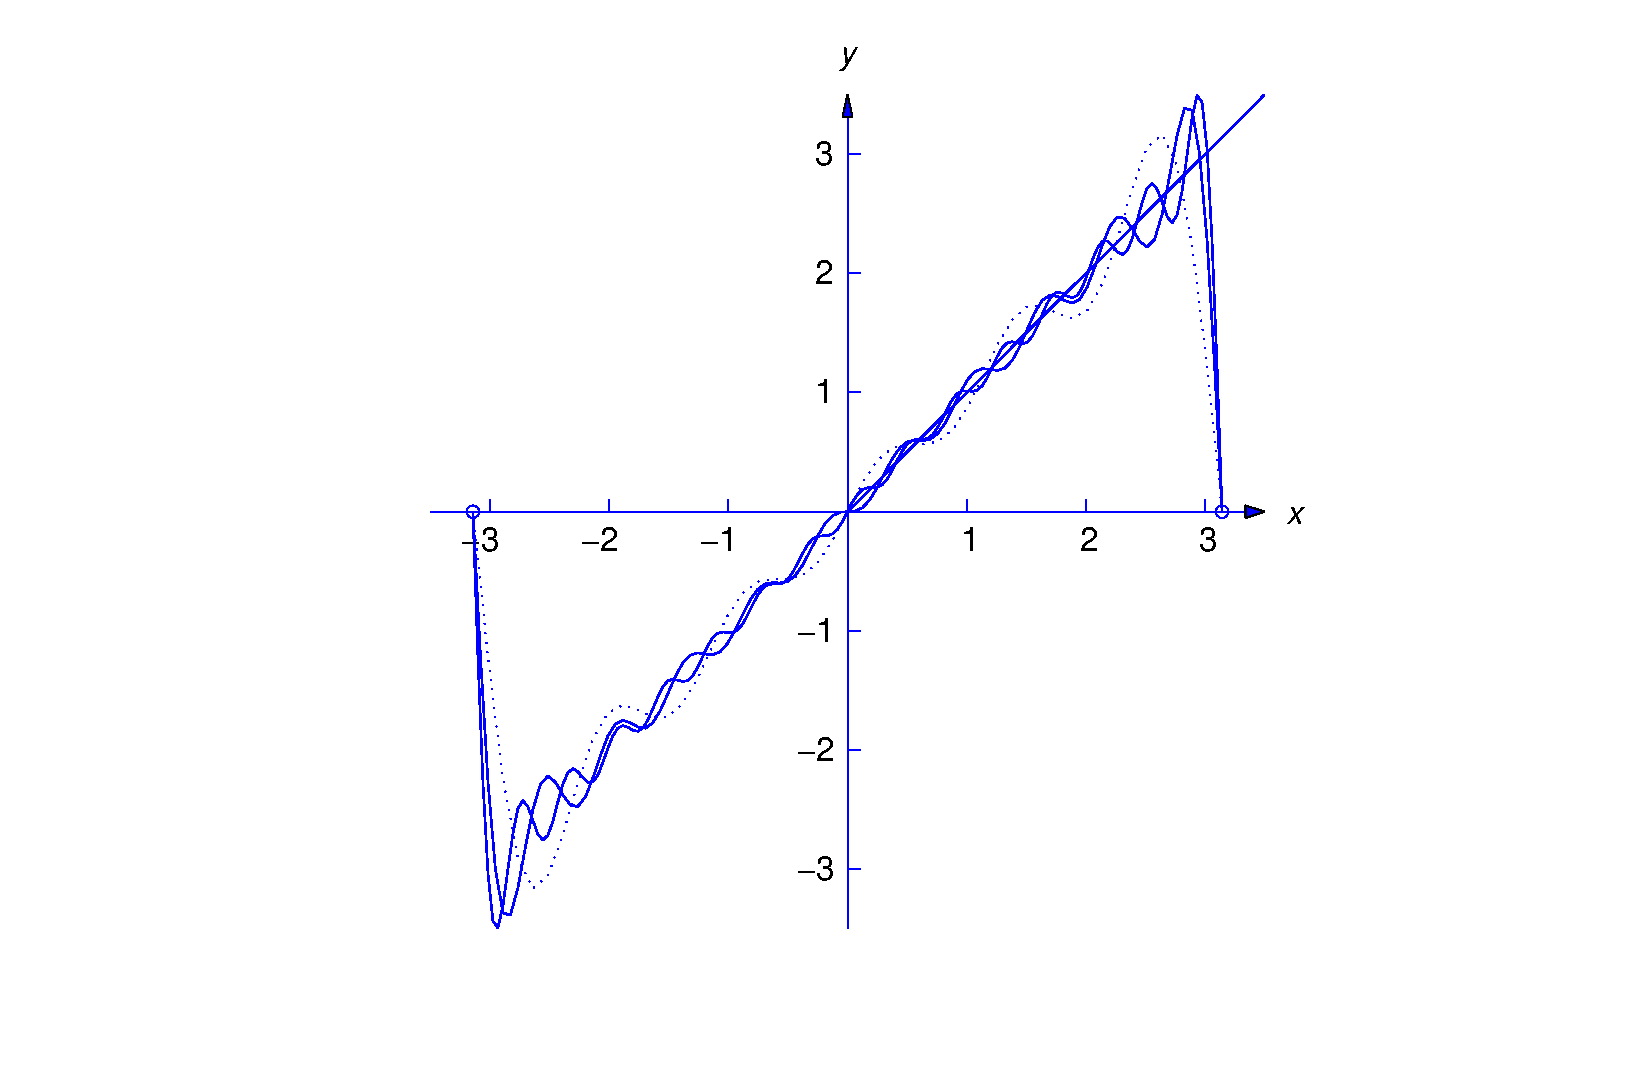
\includegraphics[bb=-78 148 689 643,width=5.67in,height=3.66in,keepaspectratio]{fig110204}
\caption{Approximation of $f(x)=x$ by partial sums
of its Fourier series on $[-\pi,\pi]$}
  \label{figure:11.2.4}
\end{figure}

\begin{example}\label{example:11.2.5} \rm
Find the Fourier series of $f(x)=|x|$ on $[-\pi,\pi]$ and
determine its sum for\\ $-\pi\le x\le\pi$.
\end{example}

\solution
Since $f$ is even and $L=\pi$,
$$
F(x)=a_0+\sum_{n=1}^\infty a_n\cos nx.
$$
Since $f(x)=x$ if $x\ge0$,
$$
a_0={1\over\pi}\int_0^\pi x\,dx={x^2\over2\pi}\lims0\pi={\pi\over2}
$$
and, if $n\ge1$,
\begin{eqnarray*}
a_n&=&{2\over\pi}\int_0^\pi x\cos nx\,dx={2\over n\pi}\left[x\sin
nx\lims0\pi-\int_0^\pi\sin nx\,dx\right]\\
&=&{2\over n^2\pi}\cos
nx\lims0\pi=\frac{2}{n^2\pi}(\cos n\pi-1)={2\over n^2\pi}[(-1)^n-1].
\end{eqnarray*}
Therefore
\begin{equation} \label{eq:11.2.12}
F(x)={\pi\over2}+{2\over\pi}\sum_{n=0}{(-1)^n-1\over n^2}\cos nx.
\end{equation}
However, since
$$
(-1)^n-1=
\left\{\begin{array}{rl} 0&\mbox{ if }n=2m,\\
-2&\mbox{ if }n=2m+1,
\end{array}\right.
$$
the terms in  \eqref{eq:11.2.12} for which $n=2m$ are all zeros.
Therefore we only to include the terms for which $n=2m+1$;
that is, we can rewrite \eqref{eq:11.2.12} as
$$
F(x)={\pi\over2}-{4\over\pi}\sum_{m=0}^\infty {1\over(2m+1)^2}
\cos(2m+1)x.
$$
However, since the name of the index of summation doesn't matter,
we prefer to replace $m$ by $n$, and write
$$
F(x)={\pi\over2}-{4\over\pi}\sum_{n=0}^\infty {1\over(2n+1)^2}
\cos(2n+1)x.
$$
Since $|x|$ is continuous for all $x$ and $|-\pi|=|\pi|$,
Theorem~\ref{thmtype:11.2.4} implies that $F(x)=|x|$ for
all $x$ in $[-\pi,\pi]$.

\begin{example}\label{example:11.2.6} \rm
Find the Fourier series of $f(x)=x(x^2-L^2)$  on $[-L,L]$,
and determine its sum for $-L\le x\le L$.
\end{example}

\solution
Since $f$ is odd,
$$
F(x)=\sum_{n=1}^\infty b_n\sin\frac{n\pi x}{L},
$$
where
\begin{eqnarray*}
b_n&=&{2\over L}\int_0^Lx(x^2-L^2)\sin{n\pi x\over L}\,dx\\
&=&-{2\over n\pi}\left[x(x^2-L^2)\cos{n\pi x\over L}\lims0L-
\int_0^L
(3x^2-L^2)\cos{n\pi x\over L}\,dx\right]\\
&=&{2L\over n^2\pi^2}\left[(3x^2-L^2)\sin{n\pi x\over
L}\lims0L-6
\int_0^Lx\sin{n\pi x\over L}\,dx\right]\\
&=&{12L^2\over n^3\pi^3}\left[x\cos{n\pi x\over L}\lims0L-
\int_0^L\cos{n\pi x\over L}\,dx\right]
=(-1)^n{12L^3\over n^3\pi^3}.
\end{eqnarray*}
Therefore
$$
F(x)={12L^3\over\pi^3}\sum_{n=1}^\infty{(-1)^n\over n^3}\sin{n\pi
x\over L}.
$$
Theorem~\ref{thmtype:11.2.4} implies that $F(x)=x(x^2-L^2)$ for all $x$
in $[-L,L]$.

\begin{example}[Gibbs Phenomenon]\label{example:11.2.7}\rm
The Fourier series of
$$
f(x)=\left\{\begin{array}{cl}
0,&-1<x<-{1\over2},\\
1,&-{1\over2}<x<{1\over2},\\[2\jot]
0,&\phantom{-}{1\over2}<x<1
\end{array}\right.
$$
on $[-1,1]$ is
$$
F(x)={1\over2}+{2\over\pi}\sum_{n=1}^\infty
{(-1)^{n-1}\over2n-1}\cos(2n-1)\pi x.
$$
(Verify.) According to Theorem~\ref{thmtype:11.2.4},
$$
F(x)=\left\{\begin{array}{cl}
0,&-1\le x<-{1\over2},\\
{1\over2},& x=-{1\over2},\\
1,&-{1\over2}<x<{1\over2},\\
{1\over2},& x={1\over2},\\
0,&{1\over2}<x\le 1;
\end{array}\right.
$$
thus, $F$ (as well as $f$) has unit jump discontinuities
at $x=\pm\frac{1}{2}$.
Figures~\ref{figure:11.2.5}-\ref{figure:11.2.7} show the graphs
of $y=f(x)$ and
$$
y=F_{2N-1}(x)=\frac{1}{2}+
{2\over\pi}\sum_{n=1}^N {(-1)^{n-1}\over2n-1}\cos(2n-1)\pi x
$$
for $N=10$, $20$, and $30$. You can see that although $F_{2N-1}$
approximates $F$ (and therefore $f$) well on larger intervals as $N$
increases, the maximum absolute values of the errors
remain approximately equal to $.09$, but occur closer to the
discontinuities $x=\pm\frac{1}{2}$ as $N$ increases.
\end{example}

\begin{figure}[H]
\color{blue}
  \begin{minipage}[b]{0.5\linewidth}
    \centering
   \scalebox{.65}{
  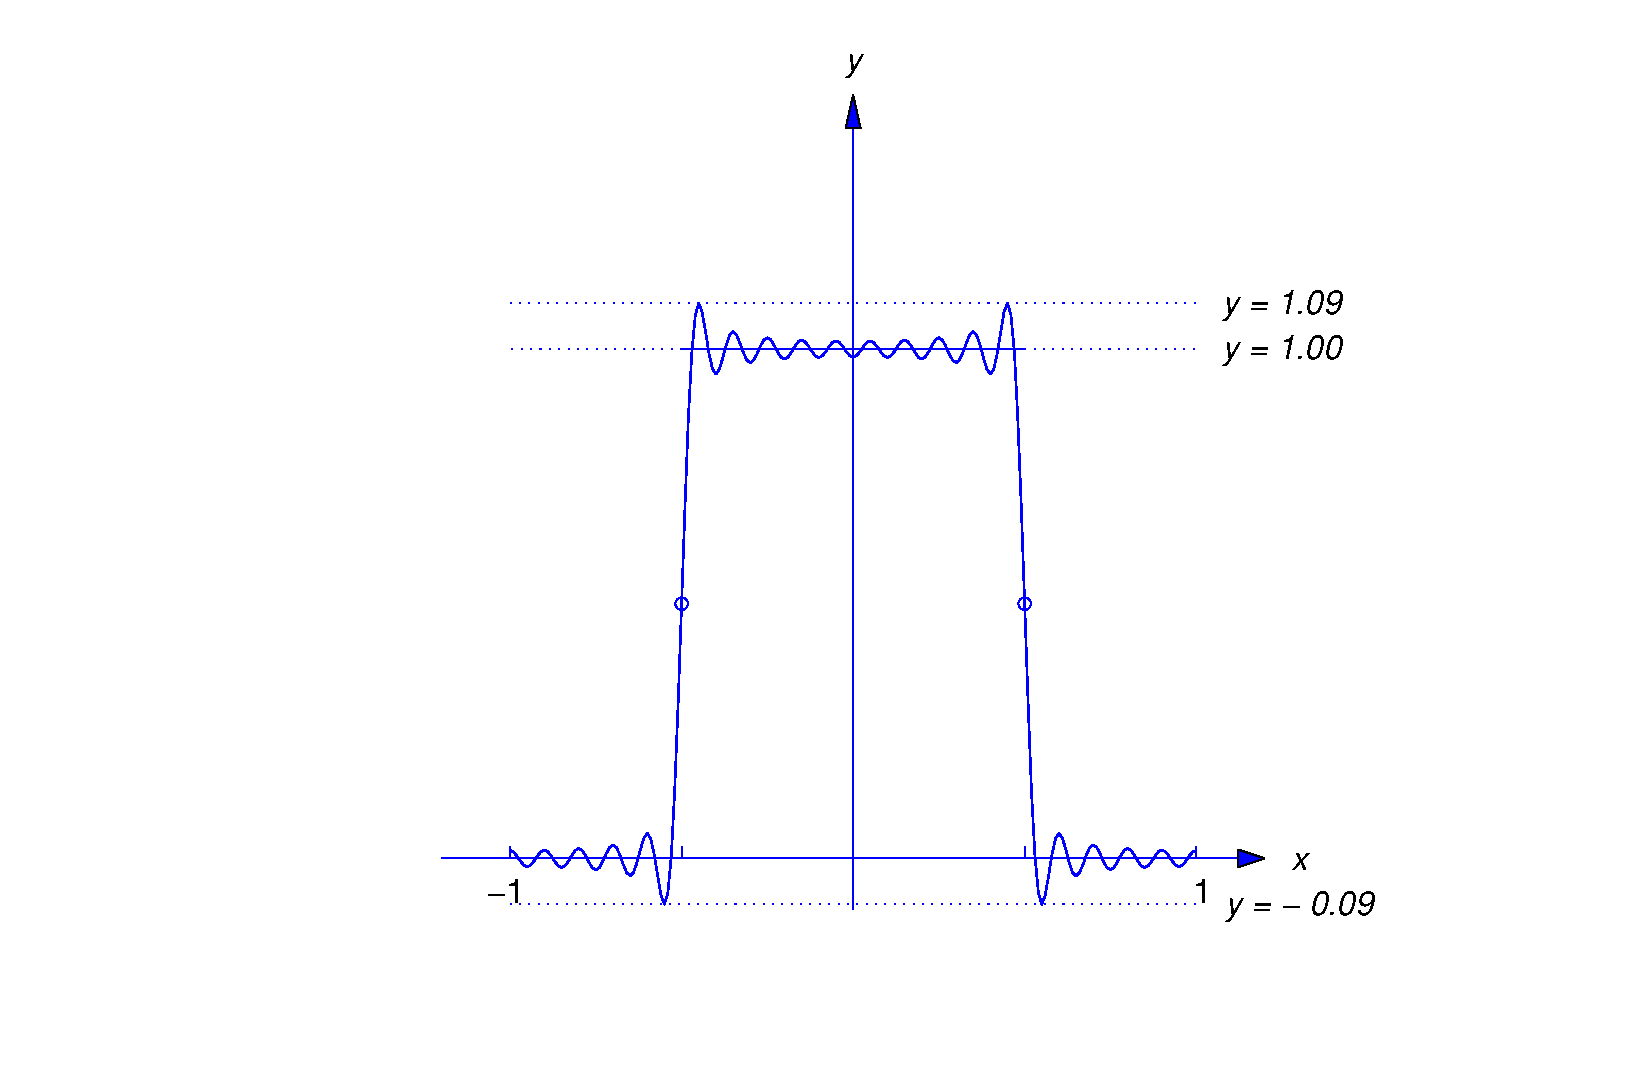
\includegraphics[bb=-78 148 689 643,width=5.67in,height=3.66in,keepaspectratio]{fig110205}}
\caption{ The Gibbs Phenomenon:
Example~\ref{example:11.2.7}, $N=10$}
  \label{figure:11.2.5}
\end{minipage}
  \begin{minipage}[b]{0.5\linewidth}
    \centering
   \scalebox{.65}{
  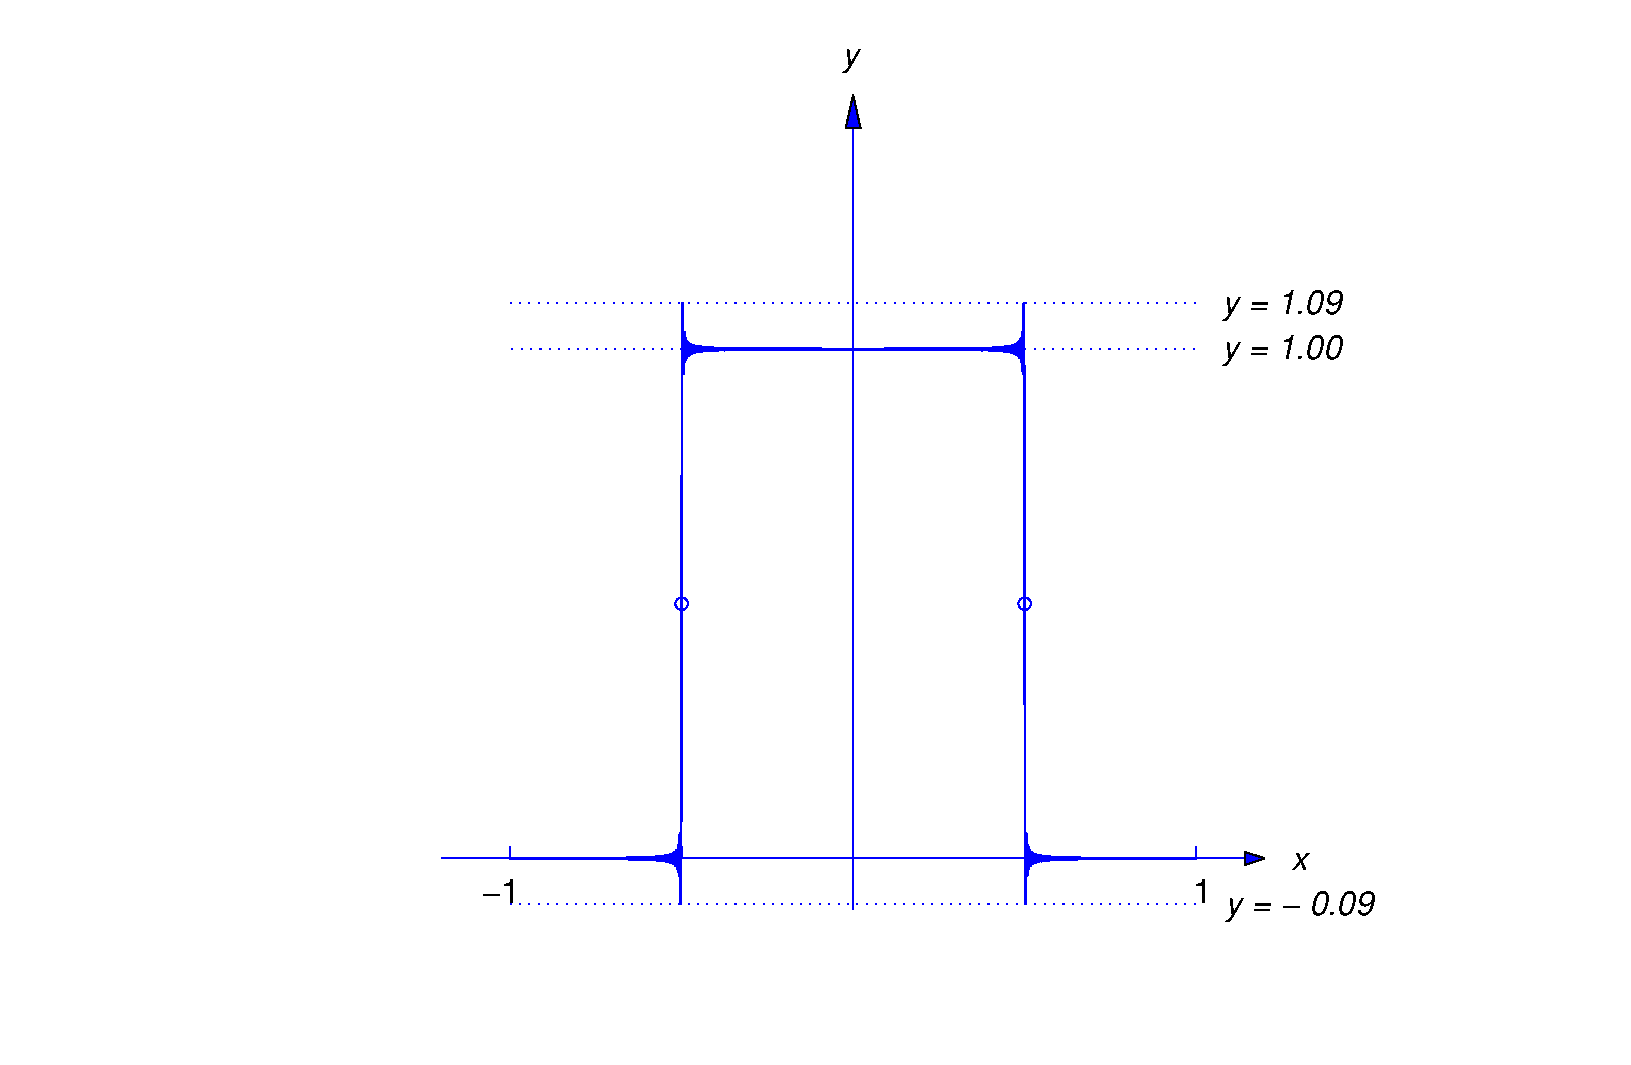
\includegraphics[bb=-78 148 689 643,width=5.67in,height=3.66in,keepaspectratio]{fig110206}}
\caption{ The Gibbs Phenomenon:
Example~\ref{example:11.2.7}, $N=20$}
  \label{figure:11.2.6}
\end{minipage}
\end{figure}

\newpage

\begin{figure}[H]
  \centering
  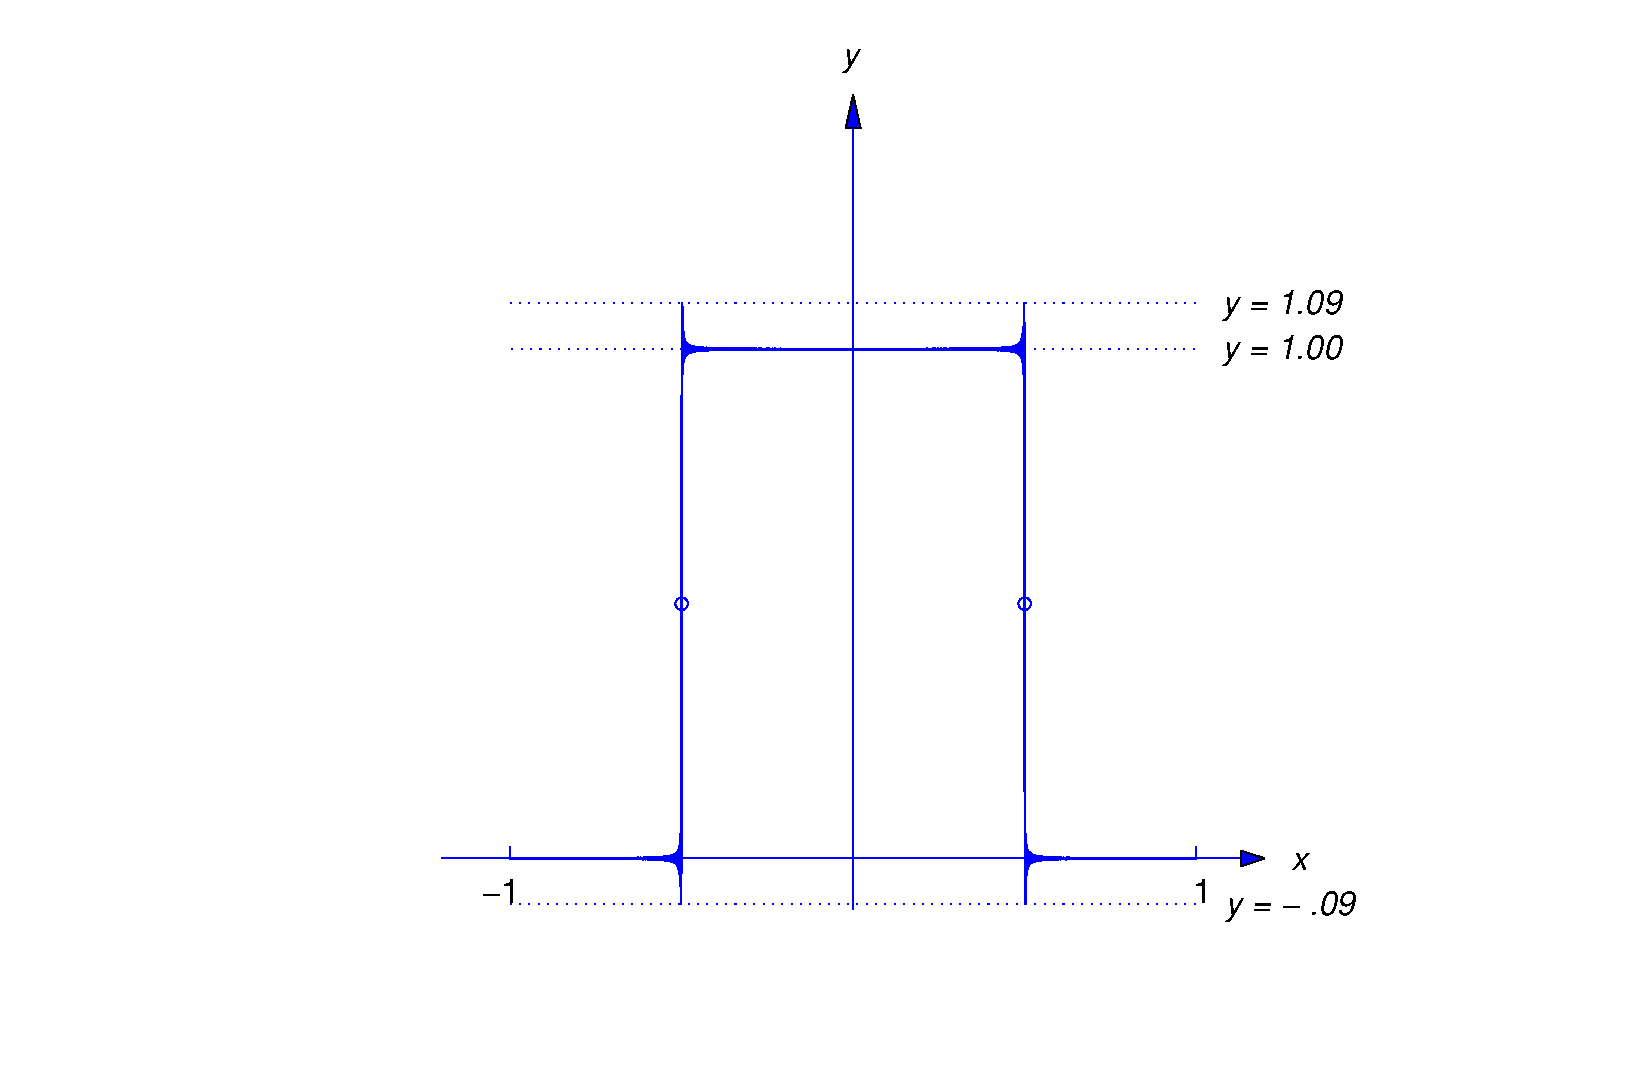
\includegraphics[bb=-78 148 689 643,width=5.67in,height=3.66in,keepaspectratio]{fig110207}
\caption{ The Gibbs Phenomenon:
Example~\ref{example:11.2.7}, $N=30$}
  \label{figure:11.2.7}
\end{figure}

\technology
\medskip

The computation of Fourier coefficients will be tedious in many of the
exercises in this chapter and the next. To learn the technique, we
recommend that you do some exercises in each section ``by hand,''
perhaps using the table of integrals at the front of the book.
However, we encourage you to use your favorite symbolic computation
software in the more difficult problems.

\exercises

\begin{exerciselist}

\item\label{exer:11.2.1}
Prove Theorem~\ref{thmtype:11.1.5}.

\exercisetext{
In Exercises~\ref{exer:11.2.2}-\ref{exer:11.2.16} find the Fourier
series of $f$ on  $[-L,L]$ and determine its sum for $-L\le x\le L$.
Where indicated by \Cex,
 graph $f$ and
$$
F_m(x)=a_0+\sum_{n=1}^m\left(a_n\cos{n\pi x\over
L}+b_n\sin{n\pi x\over L}\right)
$$
on the same axes for various values of $m$.}

\item\label{exer:11.2.2} \Cex
$L=1$;  \quad $f(x)=2-x$

\item\label{exer:11.2.3}
$L=\pi$;  \quad$f(x)=2x-3x^2$

\item\label{exer:11.2.4}
$L=1$;  \quad$f(x)=1-3x^2$

\item\label{exer:11.2.5}
$L=\pi$;  \quad$f(x)=|\sin x|$

\item\label{exer:11.2.6}  \Cex
$L=\pi$;  \quad$f(x)=x\cos x$

\item\label{exer:11.2.7}
$L=\pi$;  \quad$f(x)=|x|\cos x$

\item\label{exer:11.2.8} \Cex
$L=\pi$;  \quad$f(x)=x\sin x$

\item\label{exer:11.2.9}
$L=\pi$;  \quad$f(x)=|x|\sin x$

\item\label{exer:11.2.10}
$L=1$;  \quad$f(x)=
\left\{\begin{array}{cl}
0,&-1<x<{1\over2},\\[2\jot]
\cos\pi x,&-{1\over2}<x<{1\over2},\\[2\jot]
0,&\phantom{-}{1\over2}<x<1
\end{array}\right.$

\item\label{exer:11.2.11}
$L=1$;  \quad$f(x)=
\left\{\begin{array}{cl}
0,&-1<x<{1\over2},\\[2\jot]
x\cos\pi x,&-{1\over2}<x<{1\over2},\\[2\jot]
0,&\phantom{-}{1\over2}<x<1
\end{array}\right.$

\item\label{exer:11.2.12}
$L=1$;  \quad$f(x)=
\left\{\begin{array}{cl}
0,&-1<x<{1\over2},\\[2\jot]
\sin\pi x,&-{1\over2}<x<{1\over2},\\[2\jot]
0,&\phantom{-}{1\over2}<x<1
\end{array}\right.$

\item\label{exer:11.2.13}
$L=1$;  \quad$f(x)=
\left\{\begin{array}{cl}
0,&-1<x<{1\over2},\\[2\jot]
|\sin\pi x|,&-{1\over2}<x<{1\over2},\\[2\jot]
0,&\phantom{-}{1\over2}<x<1
\end{array}\right.$

\item\label{exer:11.2.14}
$L=1$;  \quad$f(x)=
\left\{\begin{array}{cl}
0,&-1<x<{1\over2},\\[2\jot]
x\sin\pi x,&-{1\over2}<x<{1\over2},\\[2\jot]
0,&\phantom{-}{1\over2}<x<1
\end{array}\right.$

\item\label{exer:11.2.15} \Cex
$L=4$;  \quad
$f(x)=
\left\{\begin{array}{cl}
0,&-4<x<0,\\x,&\phantom{-}0<x<4
\end{array}\right.$

\item\label{exer:11.2.16} \Cex
$L=1$;  \quad $f(x)=
\left\{\begin{array}{cl}
x^2,&-1< x<0,
\\1-x^2,&\phantom{-}0<x<1
\end{array}\right.$

\item\label{exer:11.2.17} \Lex Verify the Gibbs phenomenon for
\quad $f(x)=
\left\{\begin{array}{rl}
2,&-2< x<
-1,\\1,&-1<x<1,\\-1,&\phantom{-}1< x<2.
\end{array}\right.$

\item\label{exer:11.2.18} \Lex Verify the Gibbs phenomenon for
\quad $f(x)=
\left\{\begin{array}{rl}
2,&-3< x<
-2,\\3,&-2<x<2,\\1,&\phantom{-}2< x<3.
\end{array}\right.$

\item\label{exer:11.2.19}
Deduce from  Example~\ref{example:11.2.5} that
$$
\sum_{n=0}^\infty{1\over(2n+1)^2}={\pi^2\over 8}.
$$

\item\label{exer:11.2.20}
\begin{alist}
\item % (a)
Find the Fourier series of $f(x)=e^x$ on $[-\pi,\pi]$.
\item % (b)
Deduce from  \part{a}  that
$$
\sum_{n=0}^\infty{1\over n^2+1}={\pi\coth\pi-1\over2}.
$$
 \end{alist}

\item\label{exer:11.2.21}
Find the Fourier series of $f(x)=(x-\pi)\cos x$ on $[-\pi,\pi]$.

\item\label{exer:11.2.22}
Find the Fourier series of $f(x)=(x-\pi)\sin x$ on $[-\pi,\pi]$.

\item\label{exer:11.2.23}
Find the Fourier series  of $f(x)=\sin kx$ ($k\ne$
integer) on $[-\pi,\pi]$.

\item\label{exer:11.2.24}
Find the Fourier series  of $f(x)=\cos kx$ ($k\ne$
integer) on $[-\pi,\pi]$.

\item\label{exer:11.2.25}
\begin{alist}
\item % (a)
Suppose $g'$ is continuous on $[a,b]$ and $\omega\ne0$.
Use integration by parts to show that there's a constant $M$ such
that
$$
\left|\int_a^bg(x)\cos\omega x\,dx\right|\le{M\over\omega}
\mbox{\quad and \quad}
\left|\int_a^bg(x)\sin\omega x\,dx\right|\le{M\over\omega},\quad
\omega>0.
$$
\item % (b)
Show that the conclusion of \part{a} also holds if $g$
is piecewise smooth on $[a,b]$.  (This is a special case
of
\href{http://www-history.mcs.st-and.ac.uk/Mathematicians/Riemann.html}
{\color{blue}\it Riemann's Lemma}.
\item % (c)
We say that a sequence $\{\alpha_n\}_{n=1}^\infty$  is {\color{blue}\it of
order $n^{-k}$\/} and write
$\alpha_n=O(1/n^k)$
if  there's a constant $M$ such that
$$
|\alpha_n|<{M\over n^k},\quad n=1,2,3,\dots.
$$
Let $\{a_n\}_{n=1}^\infty$ and $\{b_n\}_{n=1}^\infty$
be the Fourier coefficients of a piecewise smooth function.
Conclude from \part{b} that $a_n=O(1/n)$  and $b_n=O(1/n)$.
\end{alist}

\item\label{exer:11.2.26}
\begin{alist}
\item % (a)
Suppose $f(-L)=f(L)$, $f'(-L)=f'(L)$,  $f'$ is continuous,
and $f''$ is piecewise continuous
on $[-L,L]$.
Use Theorem~\ref{thmtype:11.2.4} and integration by parts to show that
$$
f(x)=a_0+\sum_{n=1}^\infty\left(a_n\cos{n\pi x\over L}+b_n\sin{n\pi
x\over L}\right),\quad -L\le x\le L,
$$
with
$$
a_0={1\over 2L}\int_{-L}^L f(x)\,dx,
$$
$$
a_n= -{L\over n^2\pi^2}\int_{-L}^L f''(x)\cos{n\pi
x\over L}\,dx,\mbox{\quad and \quad}
b_n=-{L\over n^2\pi^2}\int_{-L}^L f''(x)\sin{n\pi x\over
L}\,dx,\,n\ge1.
$$
\item % (b)
Show that if, in addition to the  assumptions in \part{a},  $f''$ is
continuous and $f'''$ is piecewise continuous on
$[-L,L]$, then
$$
a_n={L^2\over n^3\pi^3}\int_{-L}^Lf'''(x)\sin{n\pi x\over L}\,dx.
$$
\end{alist}

\item\label{exer:11.2.27}
Show that if $f$ is integrable on $[-L,L]$ and
$$
f(x+L)=f(x),\quad -L<x<0
$$
(Figure~\ref{figure:11.2.8}), then the Fourier series of $f$ on $[-L,L]$
has the form
$$
A_0+\sum_{n=1}^\infty\left(A_n\cos{2n\pi\over
L}+B_n\sin{2n\pi\over L}\right)
$$
where
$$
A_0={1\over L}\int_0^Lf(x)\,dx,
$$
and
$$
A_n={2\over L}\int_0^Lf(x)\cos{2n\pi x\over L}\,dx, \quad
B_n={2\over L}\int_0^Lf(x)\sin{2n\pi x\over L}\,dx,\quad
n=1,2,3,\dots.
$$

\begin{figure}[H]
\color{blue}
  \begin{minipage}[b]{0.5\linewidth}
    \centering
   \scalebox{.65}{
  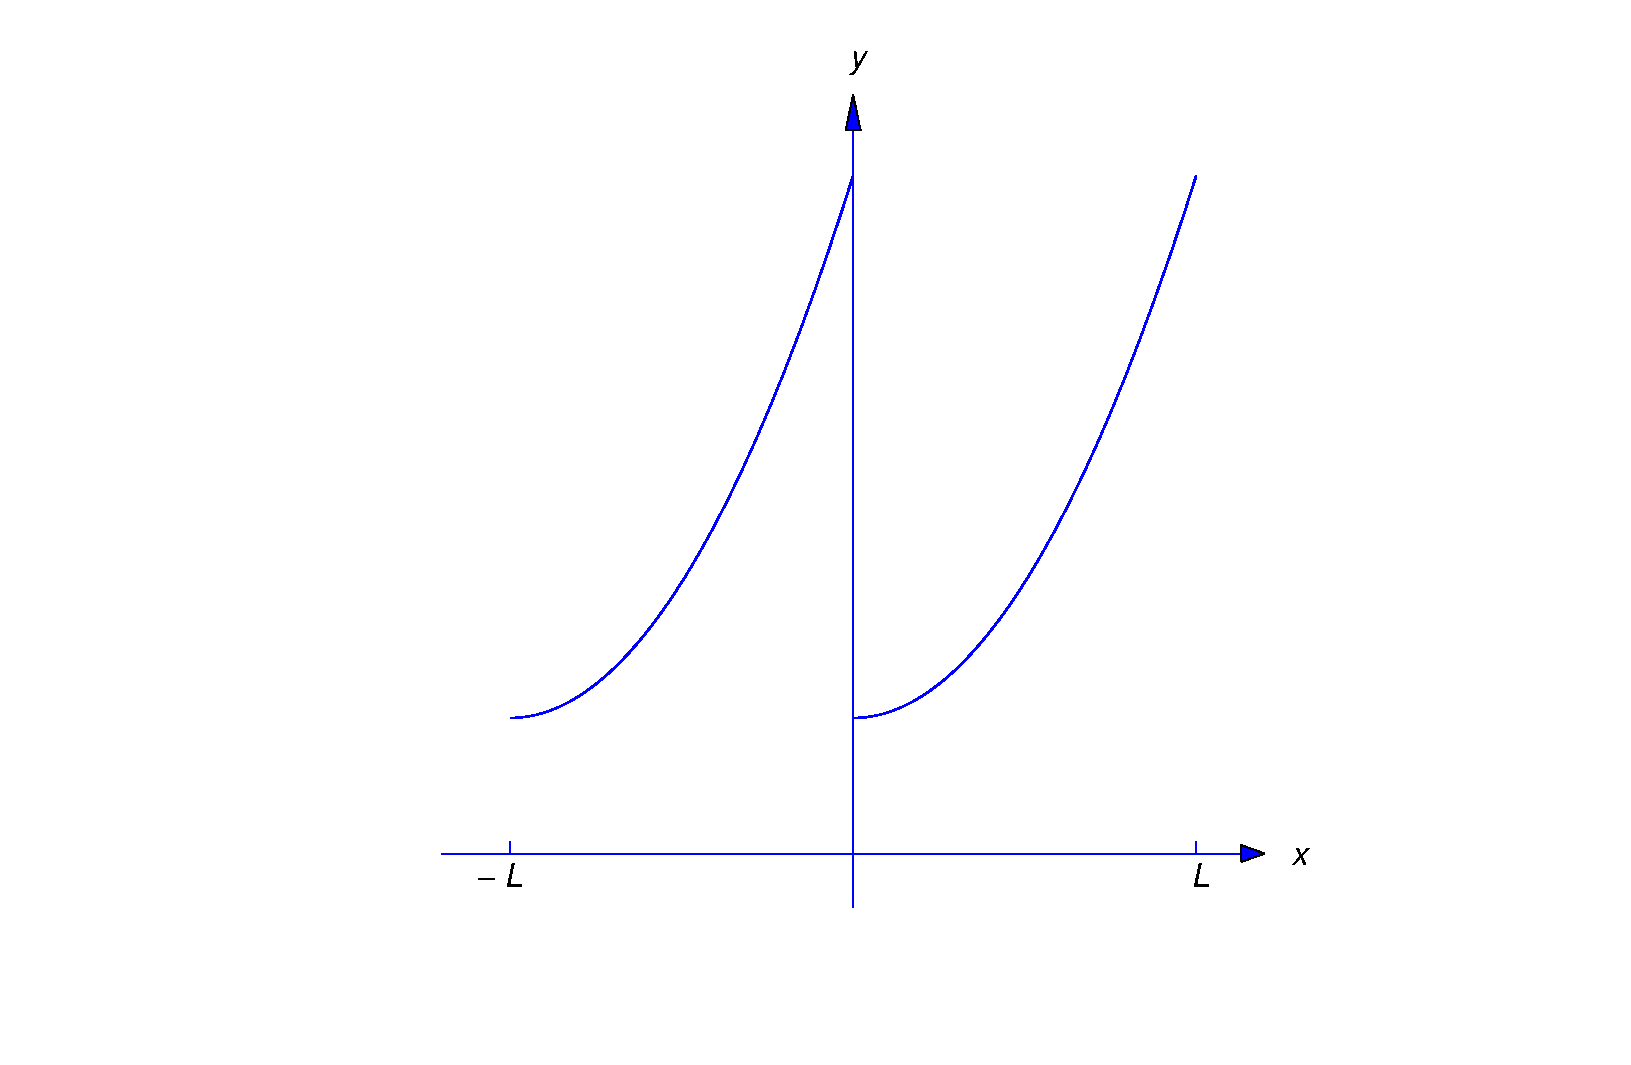
\includegraphics[bb=-78 148 689 643,width=5.67in,height=3.66in,keepaspectratio]{fig110208}}
\caption{ $y=f(x)$, where $f(x+L)=f(x)$,\, $-L<x<0$}
  \label{figure:11.2.8}
\end{minipage}
  \begin{minipage}[b]{0.5\linewidth}
    \centering
   \scalebox{.65}{
  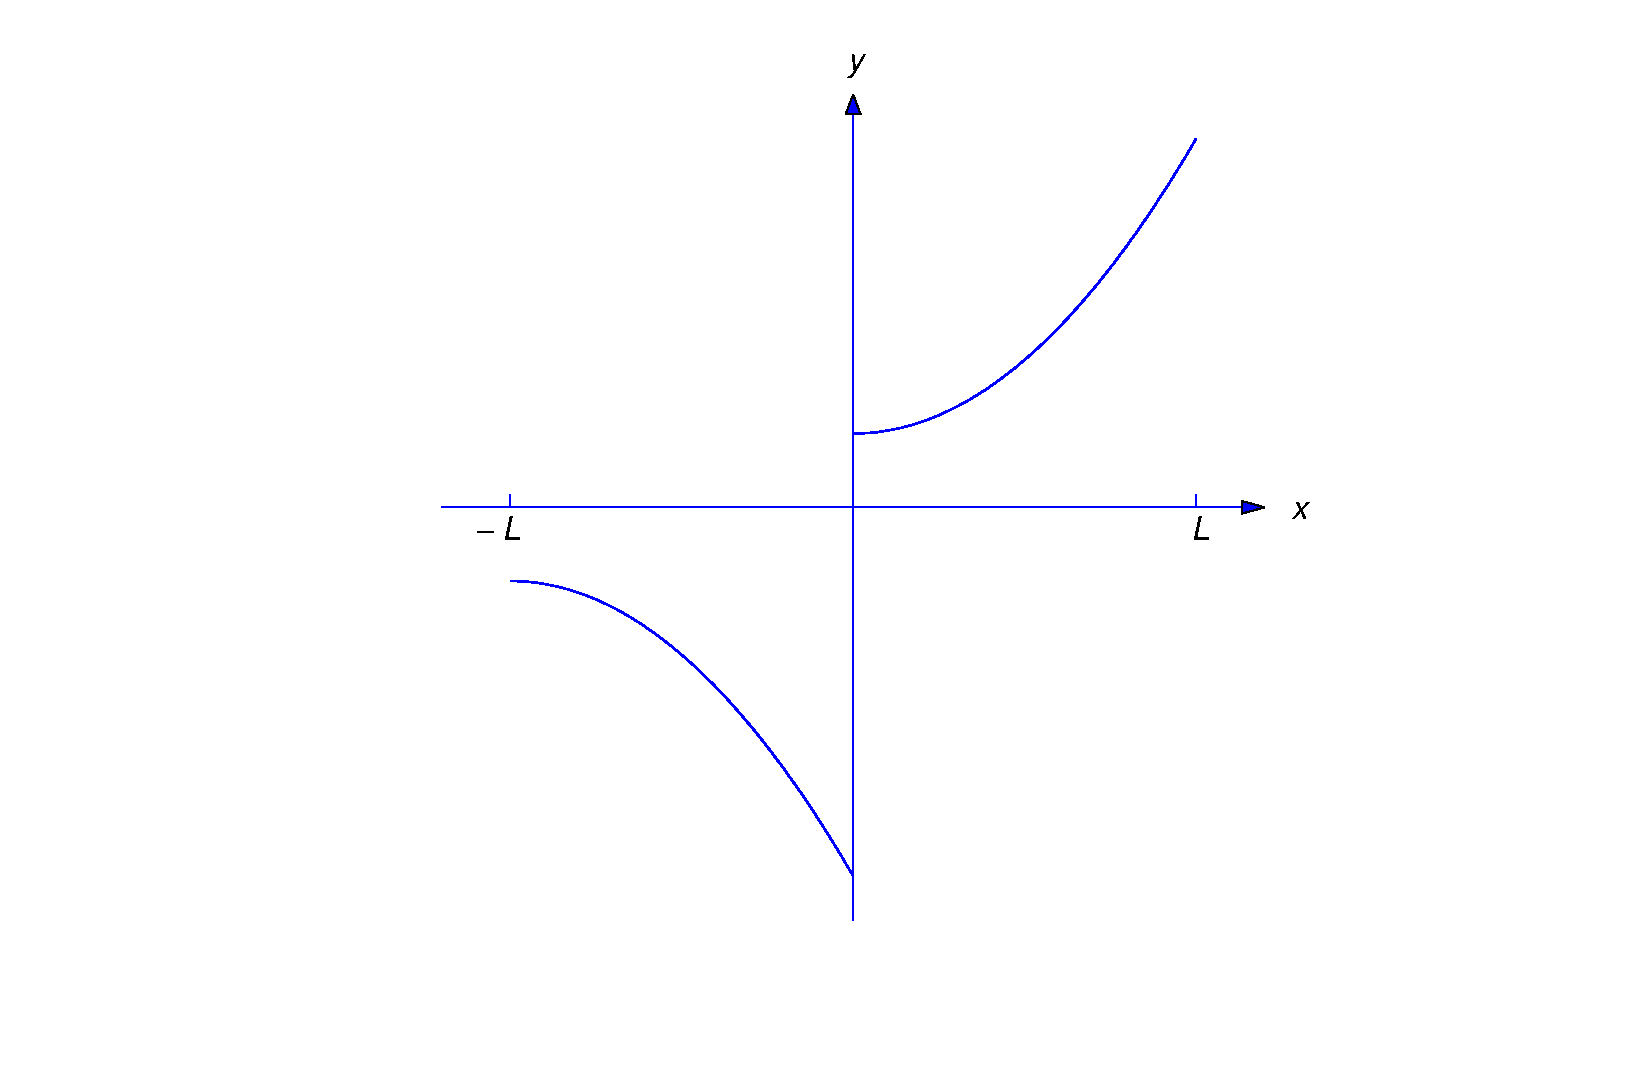
\includegraphics[bb=-78 148 689 643,width=5.67in,height=3.66in,keepaspectratio]{fig110209}}
\caption{ $y=f(x)$, where $f(x+L)=-f(x)$,
$-L<x<0$}
  \label{figure:11.2.9}
\end{minipage}
\end{figure}

\item\label{exer:11.2.28}
Show that if $f$ is integrable on $[-L,L]$ and
$$
f(x+L)=-f(x),\quad -L<x<0
$$
(Figure~\ref{figure:11.2.9}), then the Fourier series of $f$ on $[-L,L]$
has the form
$$
\sum_{n=1}^\infty\left(A_n\cos{(2n-1)\pi x\over
L}+B_n\sin{(2n-1)\pi x\over L}\right),
$$
where
$$
A_n={2\over L}\int_0^Lf(x)\cos{(2n-1)\pi x\over L}\,dx
\text{\quad and \quad }
B_n={2\over L}\int_0^Lf(x)\sin{(2n-1)\pi x\over L}\,dx,\quad
n=1,2,3,\dots.
$$

\item\label{exer:11.2.29}
Suppose $\phi_1$, $\phi_2$, \dots, $\phi_m$ are orthogonal
on $[a,b]$ and
$$
\int_a^b\phi_n^2(x)\,dx\ne0,\quad n=1,2,\dots,m.
$$
If $a_1$, $a_2$, \dots, $a_m$ are arbitrary real numbers,
define
$$
P_m=a_1\phi_1+a_2\phi_2+\cdots+a_m\phi_m.
$$
Let
$$
F_m=c_1\phi_1+c_2\phi_2+\cdots+c_m\phi_m,
$$
where
$$
c_n={\int_a^bf(x)\phi_n(x)\,dx\over\int_a^b\phi_n^2(x)\,dx};
$$
that is, $c_1$, $c_2$, \dots, $c_m$ are   Fourier coefficients of
$f$.
\begin{alist}
\item % (a)
Show that
$$
\int_a^b(f(x)-F_m(x))\phi_n(x)\,dx=0,\quad n=1,2,\dots,m.
$$
\item % (b)
Show that
$$
\int_a^b(f(x)-F_m(x))^2\,dx\le
\int_a^b(f(x)-P_m(x))^2\,dx,
$$
with equality if and only if $a_n=c_n$, $n=1,2,\dots, m$.
\item % (c)
Show that
$$
\int_a^b(f(x)-F_m(x))^2\,dx=\int_a^bf^2(x)\,dx-\sum_{n=1}^mc_n^2\int_a^b
\phi_n^2\,dx.
$$
\item % (d)
Conclude from \part{c} that
$$
\sum_{n=1}^m c_n^2\int_a^b\phi_n^2(x)\,dx\le \int_a^bf^2(x)\,dx.
$$
\end{alist}

\item\label{exer:11.2.30}
If $A_0$, $A_1$, \dots, $A_m$ and $B_1$, $B_2$, \dots, $B_m$
are arbitrary constants we say that
$$
P_m(x)=A_0+\sum_{n=1}^m\left(A_n\cos{n\pi x\over L}+B_n\sin{n\pi x\over L}\right)
$$
is a {\color{blue}\it trigonometric polynomial of degree $\le m$\/}.

Now let
$$
a_0+\sum_{n=1}^\infty\left(a_n\cos{n\pi x\over L}+b_n\sin{n\pi x\over L}\right)
$$
be the Fourier series of an integrable function $f$ on $[-L,L]$,
and let
$$
F_m(x)=
a_0+\sum_{n=1}^m\left(a_n\cos{n\pi x\over L}+b_n\sin{n\pi x\over L}\right).
$$
\begin{alist}
\item % (a)
Conclude from Exercise~\ref{exer:11.2.29}\part{b} that
$$
\int_{-L}^L(f(x)-F_m(x))^2\,dx\le
\int_{-L}^L(f(x)-P_m(x))^2\,dx,
$$
with equality if and only if $A_n=a_n$, $n=0$, $1$, \dots, $m$, and
$B_n=b_n$, $n=1$, $2$, \dots, $m$.
\item % (b)
Conclude from Exercise~\ref{exer:11.2.29}\part{d} that
$$
2a_0^2+\sum_{n=1}^m(a_n^2+b_n^2)\le{1\over L}\int_{-L}^Lf^2(x)\,dx
$$
for every $m\ge0$.
\item % (c)
Conclude from \part{b}  that
$\lim_{n\to\infty}a_n=\lim_{n\to\infty}b_n=0$.
\end{alist}

\end{exerciselist}
